\documentclass{standalone}
\usepackage{tikz}
\usetikzlibrary{patterns, positioning}


\begin{document}
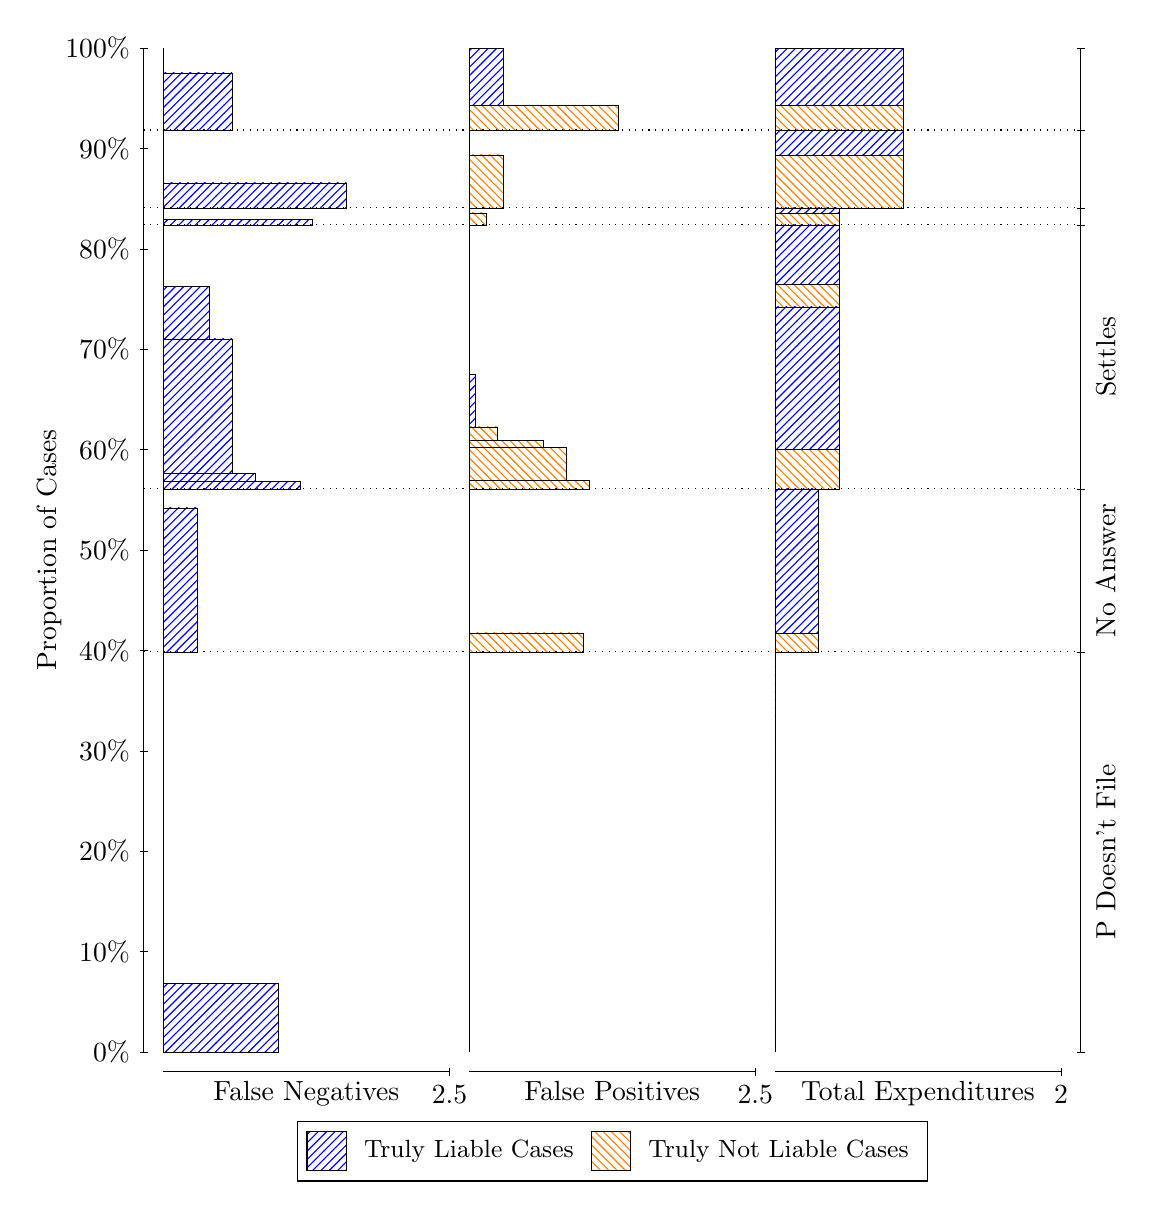
\begin{tikzpicture}
\draw[black, very thin] (1.5,1.75) -- (1.5,14.5);
\node[rotate=90, text=black, anchor=center] at (0.3, 8.125) {Proportion of Cases};
\draw[black, very thin] (1.45,1.75) -- (1.55,1.75);
\node[text=black, anchor=east] at (1.45, 1.75) {0\%};
\draw[black, very thin] (1.45,3.025) -- (1.55,3.025);
\node[text=black, anchor=east] at (1.45, 3.025) {10\%};
\draw[black, very thin] (1.45,4.3) -- (1.55,4.3);
\node[text=black, anchor=east] at (1.45, 4.3) {20\%};
\draw[black, very thin] (1.45,5.575) -- (1.55,5.575);
\node[text=black, anchor=east] at (1.45, 5.575) {30\%};
\draw[black, very thin] (1.45,6.85) -- (1.55,6.85);
\node[text=black, anchor=east] at (1.45, 6.85) {40\%};
\draw[black, very thin] (1.45,8.125) -- (1.55,8.125);
\node[text=black, anchor=east] at (1.45, 8.125) {50\%};
\draw[black, very thin] (1.45,9.4) -- (1.55,9.4);
\node[text=black, anchor=east] at (1.45, 9.4) {60\%};
\draw[black, very thin] (1.45,10.675) -- (1.55,10.675);
\node[text=black, anchor=east] at (1.45, 10.675) {70\%};
\draw[black, very thin] (1.45,11.95) -- (1.55,11.95);
\node[text=black, anchor=east] at (1.45, 11.95) {80\%};
\draw[black, very thin] (1.45,13.225) -- (1.55,13.225);
\node[text=black, anchor=east] at (1.45, 13.225) {90\%};
\draw[black, very thin] (1.45,14.5) -- (1.55,14.5);
\node[text=black, anchor=east] at (1.45, 14.5) {100\%};

\draw[black, very thin] (13.4,1.75) -- (13.4,14.5);
\draw[black, very thin] (13.35,1.75) -- (13.45,1.75);
\node[anchor=west] at (13.35, 1.75) {};
\draw[black, very thin] (13.35,6.8304) -- (13.45,6.8304);
\node[anchor=west] at (13.35, 6.8304) {};
\draw[black, very thin] (13.35,8.9018) -- (13.45,8.9018);
\node[anchor=west] at (13.35, 8.9018) {};
\draw[black, very thin] (13.35,12.255) -- (13.45,12.255);
\node[anchor=west] at (13.35, 12.255) {};
\draw[black, very thin] (13.35,12.47) -- (13.45,12.47);
\node[anchor=west] at (13.35, 12.47) {};
\draw[black, very thin] (13.35,13.459) -- (13.45,13.459);
\node[anchor=west] at (13.35, 13.459) {};
\draw[black, very thin] (13.35,14.5) -- (13.45,14.5);
\node[anchor=west] at (13.35, 14.5) {};

\draw[black, very thin, pattern color=blue, pattern=north east lines] (1.75,1.75) rectangle (3.2033,2.6245);
\draw[black, very thin, pattern color=orange, pattern=north west lines] (1.75,2.6245) rectangle (1.75,6.8304);
\draw[black, very thin, pattern color=blue, pattern=north east lines] (1.75,6.8304) rectangle (2.186,8.6586);
\draw[black, very thin, pattern color=orange, pattern=north west lines] (1.75,8.6586) rectangle (1.75,8.9018);
\draw[black, very thin, pattern color=blue, pattern=north east lines] (1.75,8.9018) rectangle (3.494,8.9993);
\draw[black, very thin, pattern color=blue, pattern=north east lines] (1.75,8.9993) rectangle (2.9127,9.0999);
\draw[black, very thin, pattern color=blue, pattern=north east lines] (1.75,9.0999) rectangle (2.622,10.807);
\draw[black, very thin, pattern color=blue, pattern=north east lines] (1.75,10.807) rectangle (2.3313,11.468);
\draw[black, very thin, pattern color=orange, pattern=north west lines] (1.75,11.468) rectangle (1.75,12.255);
\draw[black, very thin, pattern color=blue, pattern=north east lines] (1.75,12.255) rectangle (3.6393,12.32);
\draw[black, very thin, pattern color=orange, pattern=north west lines] (1.75,12.32) rectangle (1.75,12.47);
\draw[black, very thin, pattern color=blue, pattern=north east lines] (1.75,12.47) rectangle (4.0753,12.786);
\draw[black, very thin, pattern color=orange, pattern=north west lines] (1.75,12.786) rectangle (1.75,13.459);
\draw[black, very thin, pattern color=blue, pattern=north east lines] (1.75,13.459) rectangle (2.622,14.183);
\draw[black, very thin, pattern color=orange, pattern=north west lines] (1.75,14.183) rectangle (1.75,14.5);
\draw[black, very thin, pattern color=orange, pattern=north west lines] (5.6333,1.75) rectangle (5.6333,5.9559);
\draw[black, very thin, pattern color=blue, pattern=north east lines] (5.6333,5.9559) rectangle (5.6333,6.8304);
\draw[black, very thin, pattern color=orange, pattern=north west lines] (5.6333,6.8304) rectangle (7.0867,7.0736);
\draw[black, very thin, pattern color=blue, pattern=north east lines] (5.6333,7.0736) rectangle (5.6333,8.9018);
\draw[black, very thin, pattern color=orange, pattern=north west lines] (5.6333,8.9018) rectangle (7.1593,9.0121);
\draw[black, very thin, pattern color=orange, pattern=north west lines] (5.6333,9.0121) rectangle (6.8687,9.4258);
\draw[black, very thin, pattern color=orange, pattern=north west lines] (5.6333,9.4258) rectangle (6.578,9.5162);
\draw[black, very thin, pattern color=orange, pattern=north west lines] (5.6333,9.5162) rectangle (5.9967,9.6889);
\draw[black, very thin, pattern color=blue, pattern=north east lines] (5.6333,9.6889) rectangle (5.706,10.351);
\draw[black, very thin, pattern color=blue, pattern=north east lines] (5.6333,10.351) rectangle (5.6333,12.255);
\draw[black, very thin, pattern color=orange, pattern=north west lines] (5.6333,12.255) rectangle (5.8513,12.405);
\draw[black, very thin, pattern color=blue, pattern=north east lines] (5.6333,12.405) rectangle (5.6333,12.47);
\draw[black, very thin, pattern color=orange, pattern=north west lines] (5.6333,12.47) rectangle (6.0693,13.142);
\draw[black, very thin, pattern color=blue, pattern=north east lines] (5.6333,13.142) rectangle (5.6333,13.459);
\draw[black, very thin, pattern color=orange, pattern=north west lines] (5.6333,13.459) rectangle (7.5227,13.776);
\draw[black, very thin, pattern color=blue, pattern=north east lines] (5.6333,13.776) rectangle (6.0693,14.5);
\draw[black, very thin, pattern color=orange, pattern=north west lines] (9.5167,1.75) rectangle (9.5167,5.9559);
\draw[black, very thin, pattern color=blue, pattern=north east lines] (9.5167,5.9559) rectangle (9.5167,6.8304);
\draw[black, very thin, pattern color=orange, pattern=north west lines] (9.5167,6.8304) rectangle (10.062,7.0736);
\draw[black, very thin, pattern color=blue, pattern=north east lines] (9.5167,7.0736) rectangle (10.062,8.9018);
\draw[black, very thin, pattern color=orange, pattern=north west lines] (9.5167,8.9018) rectangle (10.334,9.4059);
\draw[black, very thin, pattern color=blue, pattern=north east lines] (9.5167,9.4059) rectangle (10.334,11.213);
\draw[black, very thin, pattern color=orange, pattern=north west lines] (9.5167,11.213) rectangle (10.334,11.496);
\draw[black, very thin, pattern color=blue, pattern=north east lines] (9.5167,11.496) rectangle (10.334,12.255);
\draw[black, very thin, pattern color=orange, pattern=north west lines] (9.5167,12.255) rectangle (10.334,12.405);
\draw[black, very thin, pattern color=blue, pattern=north east lines] (9.5167,12.405) rectangle (10.334,12.47);
\draw[black, very thin, pattern color=orange, pattern=north west lines] (9.5167,12.47) rectangle (11.152,13.142);
\draw[black, very thin, pattern color=blue, pattern=north east lines] (9.5167,13.142) rectangle (11.152,13.459);
\draw[black, very thin, pattern color=orange, pattern=north west lines] (9.5167,13.459) rectangle (11.152,13.776);
\draw[black, very thin, pattern color=blue, pattern=north east lines] (9.5167,13.776) rectangle (11.152,14.5);
\draw[black, dotted] (1.5,6.8304) -- (13.4,6.8304);
\draw[black, dotted] (1.5,8.9018) -- (13.4,8.9018);
\draw[black, dotted] (1.5,12.255) -- (13.4,12.255);
\draw[black, dotted] (1.5,12.47) -- (13.4,12.47);
\draw[black, dotted] (1.5,13.459) -- (13.4,13.459);
\draw[black, very thin] (1.75,1.5) -- (5.3833,1.5);
\node[text=black, anchor=north] at (3.5667, 1.5) {False Negatives};
\draw[black, very thin] (5.3833,1.45) -- (5.3833,1.55);
\node[text=black, anchor=north] at (5.3833, 1.45) {2.5};

\draw[black, very thin] (5.6333,1.5) -- (9.2667,1.5);
\node[text=black, anchor=north] at (7.45, 1.5) {False Positives};
\draw[black, very thin] (9.2667,1.45) -- (9.2667,1.55);
\node[text=black, anchor=north] at (9.2667, 1.45) {2.5};

\draw[black, very thin] (9.5167,1.5) -- (13.15,1.5);
\node[text=black, anchor=north] at (11.333, 1.5) {Total Expenditures};
\draw[black, very thin] (13.15,1.45) -- (13.15,1.55);
\node[text=black, anchor=north] at (13.15, 1.45) {2};

\node[text=black, centered, rotate=90] at (13.72, 4.2902) {P Doesn't File};
\node[text=black, centered, rotate=90] at (13.72, 7.8661) {No Answer};
\node[text=black, centered, rotate=90] at (13.72, 10.579) {Settles};




\draw (7.449999999999999,1.5) node[draw=none] (baseCoordinate) {};
\begin{scope}[align=center]
        \matrix[scale=0.5, draw=black, below=0.5cm of baseCoordinate, nodes={draw}, column sep=0.1cm]{
            \node[rectangle, draw, minimum width=0.5cm, minimum height=0.5cm, pattern color=blue, pattern=north east lines] {}; &
            \node[draw=none, font=\small, text=black] (B) {Truly Liable Cases}; &
            \node[rectangle, draw, minimum width=0.5cm, minimum height=0.5cm, pattern color=orange, pattern=north west lines] {}; &
            \node[draw=none, font=\small, text=black] (B) {Truly Not Liable Cases}; \\
            };
\end{scope}

\end{tikzpicture}
\end{document}